% Intended LaTeX compiler: pdflatex
\documentclass[10pt,a4paper,UTF8]{article}
\usepackage{zclorg}
\usepackage{tikztheorem}
\author{张朝龙}
\date{}
\title{矩阵梯度}
\hypersetup{
 pdfauthor={张朝龙},
 pdftitle={矩阵梯度},
 pdfkeywords={},
 pdfsubject={},
 pdfcreator={Emacs 25.0.50.1 (Org mode 9.0.6)},
 pdflang={English}}
\begin{document}

\maketitle
\tableofcontents
\titlepic{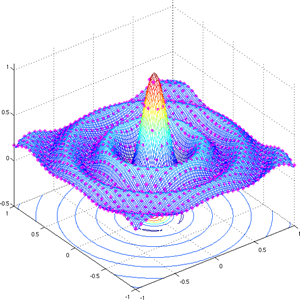
\includegraphics[scale=0.25]{../../img/sinc.PNG}}

\section{简介}
\label{sec:org58bab04}


在信息论或者机器学习的论文中,有很多黑体矢量的微分或者积分,再加上梯度函数,简直让人眼花缭乱。于是下定决心把这些黑体的矩阵语言仔细学习一下。出来混迟早是要还的,记得在大学的时候这个矩阵语言属于三不管:数学分析和线性代数都不管,其他课程就更不管了。今天属于还债日。

\section{实值函数相对于实向量的梯度}
\label{sec:orgb6e2cb8}


相对于\(n\times 1\)向量\(\mathbf{x}\)的梯度算子记作\(\nabla_{\mathbf{x}}\),定义为:
\begin{equation}
\label{eq:1}
\nabla_{\mathbf{x}} = \bigg[\frac{\partial}{\partial x_{1}}, \frac{\partial}{\partial x_{2}}, \ldots ,\frac{\partial}{\partial x_{n}} \bigg]^{T} = \frac{\partial}{\partial \mathbf{x}}
\end{equation}

因此,\(n\times 1\)实向量\(\mathbf{x}\)为变元的实标量函数\(f(\mathbf{x})\)相对于\(\mathbf{x}\)的梯度为一\(n\times 1\)的列向量,定义为:
\begin{equation}
\label{eq:2}
\nabla_{\mathbf{x}} f(\mathbf{x}) = \bigg[\frac{\partial f(\mathbf{x})}{\partial x_{1}}, \frac{\partial  f(\mathbf{x})}{\partial x_{2}}, \ldots ,\frac{\partial  f(\mathbf{x})}{\partial x_{n}} \bigg]^{T} = \frac{\partial  f(\mathbf{x})}{\partial \mathbf{x}}
\end{equation}

梯度方向的负方向成为变元\(\mathbf{x}\)的梯度流(gradient flow),记为:
\begin{equation}
\label{eq:3}
\overset{\cdot}{\mathbf{x}} = -\nabla_{\mathbf{x}}f(\mathbf{x})
\end{equation}

从梯度的定义式可以看出:
\begin{enumerate}
\item 一个以向量为变元的变量函数的梯度为一向量。
\item 梯度的每个分量给出了变量函数在该分量方向上的变化率
\end{enumerate}

梯度向量最重要的性质之一是,它指出了当变元增大时函数\(f\)的最大增大率。相反,梯度的负值(负梯度)指出了当变元增大时函数\(f\)的最大减小率。根据这样一种性质,即可设计出求一函数极小值的迭代算法。

类似地,实值函数\(f(\mathbf{x})\)相对于\(1\times n\)行向量\(\mathbf{x}^{T}\)的梯度为\(1\times n\)行向量,定义为:

\begin{equation}
\label{eq:4}
\nabla_{\mathbf{x}^{T}} f(\mathbf{x}) = \bigg[\frac{\partial f(\mathbf{x})}{\partial x_{1}}, \frac{\partial  f(\mathbf{x})}{\partial x_{2}}, \ldots ,\frac{\partial  f(\mathbf{x})}{\partial x_{n}} \bigg] = \frac{\partial  f(\mathbf{x})}{\partial \mathbf{x}^{T}}
\end{equation}

\(m\)维行向量函数\(f(\mathbf{x}) = [f_{1}(\mathbf{x}), \ldots ,f_{m}(\mathbf{x}) ]\)相对于\(n\)维实向量\(x\)的梯度为一\(n\times m\)矩阵定义为:
\begin{equation}
\label{eq:5}
\frac{\partial \mathbf{f}(\mathbf{x})}{\partial \mathbf{x}} =
\begin{bmatrix}
\frac{\partial f_{1}(\mathbf{x})}{\partial x_{1}} & \frac{\partial f_{2}(\mathbf{x})}{\partial x_{1}} & \ldots &\frac{\partial f_{m}(\mathbf{x})}{\partial x_{1}} \\
\frac{\partial f_{1}(\mathbf{x})}{\partial x_{2}} & \frac{\partial f_{2}(\mathbf{x})}{\partial x_{2}} & \ldots &\frac{\partial f_{m}(\mathbf{x})}{\partial x_{2}} \\
\vdots & \vdots & \ldots & \vdots \\
\frac{\partial f_{1}(\mathbf{x})}{\partial x_{n}} & \frac{\partial f_{2}(\mathbf{x})}{\partial x_{n}} & \ldots &\frac{\partial f_{m}(\mathbf{x})}{\partial x_{n}} \\
\end{bmatrix}
= \nabla_{\mathbf{x}}\mathbf{f}(\mathbf{x})
\end{equation}

若\(m\times 1\)向量函数\(\mathbf{f}(\mathbf{x}) = \mathbf{y} = [y_{1},\ldots ,y_{m}]^{T}\),其中\(y_{1},y_{2},\ldots ,y_{m}\)是向量的标量函数,一阶梯度:
\begin{equation}
\label{eq:6}
\frac{\partial \mathbf{y}}{\partial \mathbf{x}^{T}} =
\begin{bmatrix}
\frac{\partial y_{1}}{\partial x_{1}} & \frac{\partial y_{1}}{\partial x_{2}} & \ldots & \frac{\partial y_{1}}{\partial x_{n}} \\
\frac{\partial y_{2}}{\partial x_{1}} & \frac{\partial y_{1}}{\partial x_{2}} & \ldots & \frac{\partial y_{1}}{\partial x_{n}} \\
\end{bmatrix}
\end{equation}
\(\frac{\partial \mathbf{y}}{\partial \mathbf{x}^{T}}\)是一个\(m\times n\)的矩阵,称为向量函数\(\mathbf{y} = [y_{1},y_{2},\ldots ,y_{m}]^{T}\)的Jacobi矩阵。

若\(\mathbf{f}(\mathbf{x}) = [x_{1},x_{2},\ldots ,x_{n}]\),则:
\begin{equation}
\label{eq:7}
\frac{\partial \mathbf{x}^{T}}{\partial \mathbf{x}} = \mathbf{I}
\end{equation}
这是一个非常有用的结论,将帮助我们导出更多非常有用的结论。

\begin{tikzinstance}


若\(\mathbf{A}\)和\(\mathbf{y}\)均和\(\mathbf{x}\)无关,则:
\begin{equation}
\label{eq:9}
\frac{\partial \mathbf{x}^{T}\mathbf{A}\mathbf{y}}{\partial \mathbf{x}} = \frac{\partial \mathbf{x}^{T}}{\partial \mathbf{x}}\mathbf{A}\mathbf{y} = \mathbf{A}\mathbf{y}
\end{equation}
\end{tikzinstance}

\begin{tikzinstance}


因为\(\mathbf{y}^{T}\mathbf{A}\mathbf{x} = \langle \mathbf{A}^{T}\mathbf{y},\mathbf{x} \rangle  = \langle \mathbf{x},\mathbf{A}^{T}\mathbf{y} \rangle = \mathbf{x}^{T}\mathbf{A}^{T} \mathbf{y}\),则:
\begin{equation}
\label{eq:10}
\frac{\partial \mathbf{y}^{T}\mathbf{A}\mathbf{x}}{\partial \mathbf{x}} = \mathbf{A}^{T}\mathbf{y}
\end{equation}
\end{tikzinstance}

\begin{tikzinstance}
由于:
\begin{equation}
\label{eq:11}
x^{T}\mathbf{A}\mathbf{x} = \sum_{i=1}^{n}\sum_{j=1}^{n}A_{ij}x_{i}x_{j}
\end{equation}
所以梯度\(\frac{\partial \mathbf{x}^{T}\mathbf{A}\mathbf{x}}{\partial \mathbf{x}}\)的第\(k\)个分量为:
\begin{equation}
\label{eq:12}
\bigg[ \frac{\partial \mathbf{x}^{T}\mathbf{A}\mathbf{x}}{\partial \mathbf{x}} \bigg]_{k} = \frac{\partial}{\partial x_{k}} \sum_{i=1}^{n}\sum_{j=1}^{n}A_{ij}x_{i}x_{j} = \sum_{i=1}^{n}A_{ik}x_{i} + \sum_{j=1}^{n}A_{kj}x_{j}
\end{equation}
即有:
\begin{equation}
\label{eq:13}
\frac{\partial \mathbf{x}^{T}\mathbf{A}\mathbf{x}}{\partial \mathbf{x}} = \mathbf{A}\mathbf{x} + \mathbf{A}^{T}\mathbf{x}
\end{equation}

特别的如果\(\mathbf{A}\)为对称矩阵则有:
\begin{equation}
\label{eq:14}
\frac{\partial \mathbf{x}^{T}\mathbf{A}\mathbf{x}}{\partial \mathbf{x}} = 2\mathbf{A}\mathbf{x}
\end{equation}
\end{tikzinstance}

归纳以上三个例子的结果以及其他结果,便得到实值函数\(f(\mathbf{x})\)相对于列向量\(\mathbf{x}\)的一下几个常用的梯度公式。
\begin{tikzinstance}
若\(f(\mathbf{x}) = c\)为常数,则梯度\(\frac{\partial c}{\partial \mathbf{x}} = 0\)
\end{tikzinstance}

\begin{tikzinstance}
线性法则:若\(f(\mathbf{x})\)和\(g(\mathbf{x})\)分别是向量\(\mathbf{x}\)的实值函数,\(c_{1}\)和\(c_{2}\)为实常数,则:
\begin{equation}
\label{eq:15}
\frac{\partial[c_{1}f(\mathbf{x}) + c_{2}g(\mathbf{x})]}{\partial \mathbf{x}} = c_{1}\frac{\partial f(\mathbf{x})}{\partial \mathbf{x}} + c_{2}\frac{\partial g(\mathbf{x})}{\partial \mathbf{x}}
\end{equation}
\end{tikzinstance}
\begin{tikzinstance}
乘法法则:若\(f(\mathbf{x})\)和\(g(\mathbf{x})\)都是向量\(\mathbf{x}\)的实值函数,则:
\begin{equation}
\label{eq:16}
\frac{f(\mathbf{x})g(\mathbf{x})}{\partial \mathbf{x}} = g(\mathbf{x})\frac{\partial f(\mathbf{x})}{\partial \mathbf{x}} + f(\mathbf{x}) \frac{\partial g(\mathbf{x})}{\partial \mathbf{x}}
\end{equation}
\end{tikzinstance}
\begin{tikzinstance}
商法则:若\(g(\mathbf{x})\neq 0\),则:
\begin{equation}
\label{eq:17}
\frac{\partial f(\mathbf{x})/g(\mathbf{x})}{\partial \mathbf{x}} = \frac{1}{g^{2}(\mathbf{x})}\bigg[ g(\mathbf{x})\frac{\partial f(\mathbf{x})}{\partial \mathbf{x}} - f(\mathbf{x}) \frac{\partial g(\mathbf{x})}{\partial \mathbf{x}} \bigg]
\end{equation}
\end{tikzinstance}
\begin{tikzinstance}
链式法则:若\(\mathbf{y}(\mathbf{x})\)是\(\mathbf{x}\)的向量值函数,则:
\begin{equation}
\label{eq:18}
\frac{\partial f(\mathbf{y}(\mathbf{x}))}{\partial \mathbf{x}} = \frac{\partial \mathbf{y}^{T}(\mathbf{x})}{\partial \mathbf{x}}\frac{\partial f(\mathbf{y})}{\partial \mathbf{y}}
\end{equation}
式中\(\frac{ \partial\mathbf{y}^{T}(\mathbf{x})}{\partial \mathbf{x}}\)为\(n\times n\)矩阵。
\end{tikzinstance}
\begin{tikzinstance}
若\(n\times 1\)向量\(\mathbf{a}\)与\(\mathbf{x}\)是无关的常数向量,则:
\begin{equation}
\label{eq:19}
\frac{\partial \mathbf{a}^{T}\mathbf{x}}{\partial \mathbf{x}} = \mathbf{a} \qquad \frac{\partial\mathbf{x}^{T}\mathbf{a}}{\partial \mathbf{x}} = \mathbf{a}
\end{equation}
\end{tikzinstance}
\begin{tikzinstance}
若\(n\times 1\)向量\(\mathbf{a}\)与\(\mathbf{x}\)是无关的常数向量,则:
\begin{equation}
\label{eq:20}
\frac{\partial\mathbf{a}^{T}\mathbf{y}(\mathbf{x})}{\partial \mathbf{x}} = \frac{\partial \mathbf{y}^{T}(\mathbf{x})}{\partial \mathbf{x}} \mathbf{a} \qquad \frac{\partial\mathbf{y}^{T}(\mathbf{x})\mathbf{a}}{\partial \mathbf{x}} =\frac{\partial\mathbf{y}^{T}(\mathbf{x})}{\partial \mathbf{x}} \mathbf{a}
\end{equation}
\end{tikzinstance}

\begin{tikzinstance}
若\(\mathbf{A}\)和\(\mathbf{y}\)均与\(\mathbf{x}\)无关,则:
\begin{equation}
\label{eq:21}
\frac{\partial \mathbf{x}^{T}\mathbf{A}\mathbf{y}}{\partial \mathbf{x}} = \mathbf{A}\mathbf{y} \qquad \frac{\partial \mathbf{y}^{T}\mathbf{A}\mathbf{x}}{\partial \mathbf{x}} = \mathbf{A}^{T}\mathbf{y}
\end{equation}
\end{tikzinstance}
\begin{tikzinstance}
若\(\mathbf{A}\)是与\(\mathbf{x}\)无关,而\(\mathbf{y}(\mathbf{x})\)与向量\(\mathbf{x}\)的元素有关,则:
\begin{equation}
\label{eq:22}
\frac{\partial[\mathbf{y}(\mathbf{x})]^{T} \mathbf{A}\mathbf{y}(\mathbf{x})}{\partial \mathbf{x}} = \frac{\partial[\mathbf{y}(\mathbf{x})]^{T}}{\partial \mathbf{x}}(\mathbf{A} + \mathbf{A}^{T})\mathbf{y}(\mathbf{x})
\end{equation}
\end{tikzinstance}
\begin{tikzinstance}
若\(\mathbf{A}\)是一个与向量\(\mathbf{x}\)无关的矩阵,而\(\mathbf{y}(\mathbf{x})\)和\(\mathbf{z}(\mathbf{x})\)是与向量\(\mathbf{x}\)的元素有关的列向量,则:
\begin{equation}
\label{eq:23}
\frac{[\mathbf{y}(\mathbf{x})]^{T} \mathbf{A}\mathbf{z}(\mathbf{x})}{\partial \mathbf{x}} = \frac{[\mathbf{y}(\mathbf{x})]^{T}}{\partial \mathbf{x}} \mathbf{A}\mathbf{z}(\mathbf{x}) + \frac{[\mathbf{z}(\mathbf{x})]^{T}}{\partial \mathbf{x}}\mathbf{A}^{T}\mathbf{y}(\mathbf{x})
\end{equation}
\end{tikzinstance}

\begin{tikzinstance}
令\(\mathbf{x}\)为\(n\times 1\)向量,\(\mathbf{a}\)为\(m\times 1\)常数向量,\(\mathbf{A}\)和\(\mathbf{B}\)分别为\(m\times n\)和\(m\times m\)常数矩阵,且\(\mathbf{B}\)为对称矩阵,则:
\begin{equation}
\label{eq:24}
\frac{\partial (\mathbf{a} - \mathbf{A} \mathbf{x})^{T}\mathbf{B}(\mathbf{a} - \mathbf{A}\mathbf{x})}{\partial \mathbf{x}} = -2\mathbf{A}^{T}\mathbf{B}(\mathbf{a} - \mathbf{A}\mathbf{x})
\end{equation}
\end{tikzinstance}


\section{实值函数的梯度矩阵}
\label{sec:orgfd5e4f4}


在最优化问题中,需要最优化的对象可能是某个加权矩阵。因此,有必要分析实值函数相对于矩阵变元的梯度。

实值函数\(f(\mathbf{A})\)相对于\(m\times n\)是矩阵\(\mathbf{A}\)的梯度为一\(m\times n\)矩阵,简称梯度矩阵,定义为:
\begin{equation}
\label{eq:25}
\frac{\partial f(\mathbf{A})}{\partial \mathbf{A}} =
\begin{bmatrix}
\frac{\partial f(\mathbf{A})}{\partial A_{11}} &  \frac{\partial f(\mathbf{A})}{\partial A_{12}} &  \ldots \frac{\partial f(\mathbf{A})}{\partial A_{1n}} \\
\frac{\partial f(\mathbf{A})}{\partial A_{21}} &  \frac{\partial f(\mathbf{A})}{\partial A_{22}} &  \ldots \frac{\partial f(\mathbf{A})}{\partial A_{2n}} \\
\vdots & \vdots & \ldots & \vdots \\
\frac{\partial f(\mathbf{A})}{\partial A_{m1}} &  \frac{\partial f(\mathbf{A})}{\partial A_{m2}} &  \ldots \frac{\partial f(\mathbf{A})}{\partial A_{mn}}
\end{bmatrix}
\end{equation}
式中\(A_{ij}\)是\(\mathbf{A}\)的元素。

实值函数相对于矩阵变元的梯度具有以下性质:

\begin{tikzinstance}


若\(f(\mathbf{A})  = c\)是常数,其中\(\mathbf{A}\)为\(m\times n\)矩阵,则梯度\(\frac{\partial c}{\partial \mathbf{A}} = \mathbf{O}_{m\times n}\)
\end{tikzinstance}

\begin{tikzinstance}


线性法则:若\(f(\mathbf{A})\)和\(g(\mathbf{A})\)分别是矩阵\(\mathbf{A}\)的实值函数,\(c_{1},c_{2}\)均为实常数,则:
\begin{equation}
\label{eq:26}
\frac{\partial [c_{1}f(\mathbf{A}) + c_{2}g(\mathbf{A})]}{\partial \mathbf{A}} = c_{1}\frac{\partial f(\mathbf{A})}{\partial \mathbf{A}} + c_{2}\frac{\partial g(\mathbf{A})}{\partial \mathbf{A}}
\end{equation}
\end{tikzinstance}

\begin{tikzinstance}
乘积法则:若\(f(\mathbf{A})\),\(g(\mathbf{A})\)都是矩阵\(\mathbf{A}\)的实值函数,则:
\begin{equation}
\label{eq:27}
\frac{\partial f(\mathbf{A})g(\mathbf{A})}{\partial \mathbf{A}} = f(\mathbf{A})\frac{\partial g(\mathbf{A})}{\partial \mathbf{A}} + g(\mathbf{A}) \frac{\partial f(\mathbf{A})}{\partial \mathbf{A}}
\end{equation}
\end{tikzinstance}

\begin{tikzinstance}
商法则:若\(g(\mathbf{A})\neq 0\),则:
\begin{equation}
\label{eq:28}
\frac{\partial f(\mathbf{A})/g(\mathbf{A})}{\partial \mathbf{A}} = \frac{1}{[g(\mathbf{A})]^{2}} \bigg[  g(\mathbf{A}) \frac{\partial f(\mathbf{A})}{\partial \mathbf{A}}  - f(\mathbf{A}) \frac{\partial g(\mathbf{A})}{\partial \mathbf{A}} \bigg]
\end{equation}
\end{tikzinstance}

\begin{tikzinstance}


链式法则:令\(\mathbf{A}\)为\(m\times n\)的矩阵,且\(y=f(\mathbf{A})\)和\(g(y)\)分别是以矩阵\(\mathbf{A}\)和标量\(y\)为变元的实值函数,则:
\begin{equation}
\label{eq:29}
\frac{\partial g(f(\mathbf{A}))}{\partial \mathbf{A}} = \frac{\mathrm{d}g(y)}{\mathrm{d} y}\frac{\partial f(\mathbf{A})}{\partial \mathbf{A}}
\end{equation}
\end{tikzinstance}

\begin{tikzinstance}


若\(\mathbf{A}\in R^{m\times n}\),\(\mathbf{x}\in R^{m\times 1}\),\(\mathbf{y}\in R^{n\times 1}\),则:

\begin{equation}
\label{eq:30}
\frac{\partial \mathbf{x}^{T}\mathbf{A}\mathbf{y}}{\partial \mathbf{A}} = \mathbf{x}\mathbf{y}^{T}
\end{equation}
\end{tikzinstance}

\begin{tikzinstance}


若\(\mathbf{A}\in R^{n\times n}\)非奇异,\(\mathbf{x}\in R^{n\times 1}\),\(\mathbf{y}\in R^{n\times 1}\),则:
\begin{equation}
\label{eq:31}
\frac{\partial \mathbf{x}^{T} \mathbf{A}^{-1}\mathbf{y}}{\partial \mathbf{A}} = -\mathbf{A}^{-T}\mathbf{x}\mathbf{y}^{T}\mathbf{A}^{-T}
\end{equation}
\end{tikzinstance}


\begin{tikzinstance}


若\(\mathbf{A}\in R^{m\times n},\mathbf{x}\in R^{n\times 1},\mathbf{y}\in R^{n\times 1}\),则:
\begin{equation}
\label{eq:32}
\frac{\partial \mathbf{x}^{T} \mathbf{A}^{T}\mathbf{A}\mathbf{y}}{\partial \mathbf{A}} = \mathbf{A}(\mathbf{x}\mathbf{y}^{T} + \mathbf{y}\mathbf{x}^{T})
\end{equation}
\end{tikzinstance}

\begin{tikzinstance}
若\(\mathbf{A}\in R^{m\times n},\mathbf{x},\mathbf{y}\in R^{m\times 1}\),则:
\begin{equation}
\label{eq:33}
\frac{\partial \mathbf{x}^{T}\mathbf{A}\mathbf{A}^{T}\mathbf{y}}{\partial \mathbf{A}} =  (\mathbf{x}\mathbf{y}^{T} + \mathbf{y}\mathbf{x}^{T})\mathbf{A}
\end{equation}
\end{tikzinstance}

\begin{tikzinstance}
指数函数的梯度:
\begin{equation}
\label{eq:34}
\frac{\partial \exp(\mathbf{x}^{T}\mathbf{A}\mathbf{y})}{\partial \mathbf{A}} = \mathbf{x}\mathbf{y}^{T} \exp(\mathbf{x}^{T}\mathbf{A}\mathbf{y})
\end{equation}
\end{tikzinstance}

\section{迹函数的梯度矩阵}
\label{sec:orgba1bc8d}


有时候,二次型目标函数可以利用矩阵的迹加以重写。因为一标量可以视为\(1\times 1\)的矩阵,所以二次型目标函数的迹直接等同于函数本身,即\(f(\mathbf{x}) = \mathbf{x}^{T}\mathbf{A}\mathbf{x} = \mathrm{tr}(\mathbf{x}^{T}\mathbf{A}\mathbf{x})\) 利用迹的性质,又可以将目标函数进一步表示为:
\begin{equation}
\label{eq:35}
f(\mathbf{x}) = \mathbf{x}^{T}\mathbf{A}\mathbf{x} = \mathrm{tr}(\mathbf{x}^{T}\mathbf{A}\mathbf{x}) = \mathrm{tr}(\mathbf{A}\mathbf{x}\mathbf{x}^{T})
\end{equation}

因此,二次型目标函数\(\mathbf{x}^{T}\mathbf{A}\mathbf{x}\)等于核矩阵\(\mathbf{A}\)和向量外积\(\mathbf{x}\mathbf{x}^{T}\)的乘积的迹\(\mathrm{tr}(\mathbf{A}\mathbf{x}\mathbf{x}^{T})\)

\begin{tikzinstance}


对于\(n\times n\)矩阵\(\mathbf{A}\),由于\(\mathrm{tr}(\mathbf{A}) = \sum_{i=1}^{n}A_{ii}\),故梯度\(\frac{\partial \mathrm{tr}(\mathbf{A})}{\partial \mathbf{A}}\)的\((i,j)\)元素为:
\begin{equation}
\label{eq:37}
\bigg[\frac{\partial \mathrm{tr}(\mathbf{A})}{\partial \mathbf{A}} \bigg]_{ij} = \frac{\partial}{\partial A_{ij}}\sum_{k=1}^{n}A_{kk} =
\begin{cases}
1 & j=i \\
0 & j\neq i
\end{cases}
\end{equation}
所以有\(\frac{\partial \mathrm{tr}(\mathbf{A})}{\partial \mathbf{A}} = \mathbf{I}\)
\end{tikzinstance}

\begin{tikzinstance}


考察目标函数\(f(\mathbf{A}) = \mathrm{tr}(\mathbf{A}\mathbf{B})\),其中\(\mathbf{A}\)和\(\mathbf{B}\)分别为\(m\times n\)和\(n\times m\)实矩阵。首先,矩阵乘积的元素为\([\mathbf{A}\mathbf{B}]_{ij} = \sum_{l=1}^{n}A_{il}B_{lj}\),故矩阵乘积的迹\(\mathrm{tr}(\mathbf{A}\mathbf{B}) = \sum_{p=1}^{m}\sum_{l=1}^{n}A_{pl}B_{lp}\),于是,梯度\(\frac{\partial \mathrm{tr}(\mathbf{A}\mathbf{B})}{\partial \mathbf{A}}\)是一个\(m\times n\)矩阵,其元素为:
\begin{equation}
\label{eq:38}
\bigg[ \frac{\partial \mathrm{tr}(\mathbf{A}\mathbf{B})}{\partial \mathbf{A}} \bigg]_{ij} = \frac{\partial }{\partial A_{ij}} \bigg(\sum_{p=1}^{m}\sum_{l=1}^{n}A_{pl}B_{lp} \bigg) = B_{ji}
\end{equation}
所以有:
\begin{equation}
\label{eq:39}
\frac{\partial \mathrm{tr}(\mathbf{A}\mathrm{B})}{\partial \mathbf{A}} = \nabla_{\mathbf{A}} \mathrm{tr}(\mathbf{A}\mathrm{B}) = \mathbf{B}^{T}
\end{equation}
由于\(\mathrm{tr}(\mathbf{B}\mathbf{A}) = \mathrm{tr}(\mathbf{A}\mathbf{B})\)所以:
\begin{equation}
\label{eq:40}
\frac{ \partial \mathrm{tr}(\mathbf{A}\mathrm{B}) }{\partial \mathbf{A}} = \frac{\partial \mathrm{tr}(\mathbf{B}\mathbf{A})}{\partial \mathbf{A}} = \mathbf{B}^{T}
\end{equation}
同理,由于\(\mathrm{tr}(\mathbf{x}\mathbf{y}^{T}) = \mathrm{tr}(\mathbf{y}\mathbf{x}^{T}) = \mathbf{x}^{T}\mathbf{y}\),所以有:
\begin{equation}
\label{eq:41}
\frac{\partial \mathrm{tr}(\mathbf{x}\mathbf{y}^{T})}{\partial  \mathbf{x}} = \frac{\partial \mathrm{tr}(\mathbf{y}\mathbf{x}^{T})}{\partial  \mathbf{x}} = \mathbf{y}
\end{equation}
\end{tikzinstance}

\section{Hessian矩阵}
\label{sec:org004c744}


实值函数\(f(\mathbf{x})\)相对于\(m\times 1\)实向量\(\mathbf{x}\)的二阶偏导是一个由\(m^{2}\)个二阶偏导组成的矩阵,称为Hessian矩阵,定义为:
\begin{equation}
\label{eq:42}
\frac{\partial^{2} f(\mathbf{x})}{\partial \mathbf{x} \partial \mathbf{x}^{T}} = \frac{\partial}{\partial \mathbf{x}^{T}} \bigg[\frac{\partial f(\mathbf{x})}{\partial \mathbf{x}} \bigg]
\end{equation}
或者简写为梯度的梯度:
\begin{equation}
\label{eq:43}
\nabla_{\mathbf{x}}^{2}f(\mathbf{x}) = \nabla_{\mathbf{x}} (\nabla_{\mathbf{x}} f(\mathbf{x}))
\end{equation}
根据定义,Hessian矩阵的第\(j\)列是梯度\(\frac{\partial f(\mathbf{x})}{\partial \mathbf{x}} = \nabla_{\mathbf{x}} f(\mathbf{x})\)第\(j\)个分量的梯度,即:
\begin{equation}
\label{eq:44}
\bigg[ \frac{\partial^{2}f(\mathbf{x}) }{\partial \mathbf{x} \partial \mathbf{x}^{T}} \bigg]_{i,j} = \frac{\partial^{2}f(\mathbf{x})}{\partial x_{i} \partial x_{j}}
\end{equation}
或者可以写作:
\begin{equation}
\label{eq:45}
\frac{\partial^{2} f(\mathbf{x})}{\partial \mathbf{x} \partial \mathbf{x}^{T}} =
\begin{bmatrix}
\frac{\partial^{2}f}{\partial x_{1}\partial x_{1}} & \frac{\partial^{2}f}{\partial x_{1}\partial x_{2}} & \ldots & \frac{\partial^{2}f}{\partial x_{1}\partial x_{n}} \\
\frac{\partial^{2}f}{\partial x_{2}\partial x_{1}} & \frac{\partial^{2}f}{\partial x_{2}\partial x_{2}} & \ldots & \frac{\partial^{2}f}{\partial x_{2}\partial x_{n}} \\
\vdots & \vdots & \ddots & \vdots \\
\frac{\partial^{2}f}{\partial x_{n}\partial x_{1}} & \frac{\partial^{2}f}{\partial x_{n}\partial x_{2}} & \ldots & \frac{\partial^{2}f}{\partial x_{n}\partial x_{n}} \\
\end{bmatrix}

\end{equation}
因此,Hessian矩阵可以通过两个步骤计算得出:
\begin{enumerate}
\item 求实值函数\(f(\mathbf{x})\)关于向量变元\(\mathbf{x}\)的偏导数,得到实值函数的梯度\(\frac{\partial f(\mathbf{x})}{\partial \mathbf{x}}\)
\item 再求梯度\(\frac{\partial f(\mathbf{x})}{\partial \mathbf{x}}\)相对于\(1\times n\)行向量\(\mathbf{x}^{T}\)的偏导数,得到梯度的梯度即Hessian矩阵
\end{enumerate}

根据以上步骤,得到Hessian矩阵的下列公式。
\begin{tikzinstance}
对于\(n\times 1\)的常数向量\(\mathbf{a}^{T}\),有:
\begin{equation}
\label{eq:47}
\frac{\partial^{2} \mathbf{a}^{T}\mathbf{x}}{\partial \mathbf{x}\partial \mathbf{x}^{T}} = \mathbf{O}_{n\times n}
\end{equation}
\end{tikzinstance}
\begin{tikzinstance}
若\(\mathbf{A}\)是\(n\times n\)矩阵,则:
\begin{equation}
\label{eq:48}
\frac{\partial^{2} \mathbf{x}^{T}\mathbf{A}\mathbf{x}}{\partial \mathbf{x}\partial \mathbf{x}^{T}} = \mathbf{A} + \mathbf{A}^{T}
\end{equation}
\end{tikzinstance}

\begin{tikzinstance}
令\(\mathbf{x}\)为\(n\times 1\)向量,\(\mathbf{a}\)为\(m\times 1\)常数向量,\(\mathbf{A}\)和\(\mathbf{B}\)分别为\(m\times n\)和\(m\times m\)常数矩阵,且\(\mathbf{B}\)为对称矩阵,则:
\begin{equation}
\label{eq:49}
\frac{\partial^{2}(\mathbf{a} - \mathbf{A}\mathbf{x})^{T}\mathbf{B} (\mathbf{a} - \mathbf{A}\mathbf{x}) }{\partial \mathbf{x} \partial \mathbf{x}^{T}} = 2\mathbf{A}^{T}\mathbf{B}\mathbf{A}
\end{equation}
\end{tikzinstance}
\section{尾声}
\label{sec:org9423f40}


矩阵的语言非常的丰富,如果再加上随机矩阵,则又会有更多的结论。这些仅在一篇博文中恐怕难以详述。本文只大概的给出一些经常用到的结论。在实际应用中,还要多多查阅相关书籍。
\end{document}
